\documentclass{article}

% tight measures:
% \usepackage[margin=0mm, paperwidth=56mm, paperheight=42mm]{geometry}
% loose measures:
\usepackage[margin=2mm, paperwidth=24mm, paperheight=40mm]{geometry}

\usepackage{amsmath}
\usepackage{tikz}
\usetikzlibrary{bayesnet}
\usepackage{bm}
\providecommand{\mathbold}[1]{\bm{#1}}
\newcommand{\vct}[1]{\mathbold{#1}}

\begin{document}
\thispagestyle{empty}

\begin{center}
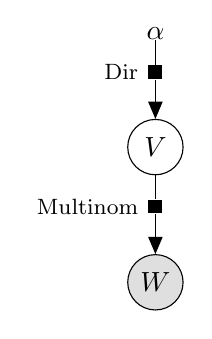
\begin{tikzpicture}
   \node[latent] (v) {$V$} ;
   \node[const, above= of v] (alp) {$\alpha$} ;
   \node[obs, below=1 of v] (N) {$W$} ;
   \factor[above=.5 of v] {alp-v} {left:Dir} {alp} {v} ;
   \factor[below=.3 of v] {v-N} {left:Multinom} {v} {N} ;
\end{tikzpicture}
\end{center}

\end{document}











